\subsection{Residual learning block}
跳跃连接,基本的残差块如Fig.\ref{fig:residual}所示(当然残差块不止有这一种形式,可以根据需求定义不同的残差块)。残差学习由何凯明基于以下问题提出:给定一个学习问题后,逐渐加深网络的层的时候,模型的效果应该是逐渐提升的或者不能低于原来模型的效果,但是在实验中发现通常加深后模型的效果反而变差了。按理来说就算不能提升了,额外增加的层也可以学习到一个恒等映射来保持效果不变啊,但是为什么反而下降了呢?这便是\textbf{模型退化问题}。

假设原本要学习的问题是$\mathcal{H}(x)$,之前的想法是直接学习它,在残差学习中,将它进行分解$\mathcal{H}(x) = \mathcal{F}(x) + x$,由于$x$是已知的,那么只需要学习$\mathcal{F}$就好了,$\mathcal{F}$也就是所说的残差。

\textbf{为什么这样会有效呢?}由于神经网络中通常都会使用非线性函数来拟合复杂的函数,但是对于线性关系却有点力不从心(可能这就是为什么不能学习到恒等映射的原因吧)。残差学习不仅保留了学习非线性函数的能力,也提高了线性函数的学习能力 --- $\mathcal{F}$为0即可。Resudial Learning的这种能力使得更深的网络称为可能。

\begin{figure}[h]
	\centering
	\includegraphics[width=.4\textwidth]{pics/Residual.png}
	\caption{Residual}
	\label{fig:residual}
\end{figure}

\subsection{Dense Connection}
稠密连接,如Fig.\ref{fig:dense block}所示。每一层与之前的所有层都有连结。用$H_l$表示第$l$层,$\boldsymbol{X}_l$表示第$l$层的输出,则$\boldsymbol{X}_l = H_l(\boldsymbol{X}_0, \boldsymbol{X}_1, ..., \boldsymbol{X}_{l-1})$。

有以下优点:1)减轻了梯度消失问题;2)加强了特征的传播,能够有效的利用学习到的特征;3)能够利用多层次的特征。
\begin{figure}[h]
	\centering
	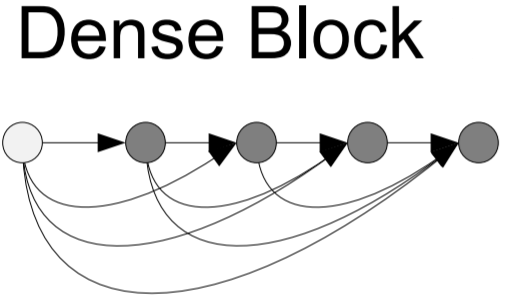
\includegraphics[width=.4\textwidth]{pics/dense block.png}
	\caption{Dense Block}
	\label{fig:dense block}
\end{figure}

\subsection{Dilated Convolution}空洞卷积。在pooling时,可以减小feature map的尺寸,也能增大每个元素的感受野但是也损失了空间信息。在进行分割时,pooling损失的那部分信息是难以复原的。dilated卷积是一种特殊的卷积,与通常的卷积不同,dilated卷积会在\textbf{卷积核元素之间插入空格},其实相当于一个更大的卷积核,而那些插入的卷积核的值一直为0。如Fig.\ref{fig:dilation}所示。Dilation卷积可以在不做pooling损失信息的情况下增大感受野,pooling虽然可以增大感受野但是失去了位置信息,难以从pooling后的层恢复到原来的信息,而dilation卷积不仅增大了感受野,还保留了特征图中元素的相对空间信息。
\begin{figure}[h]
	\centering
	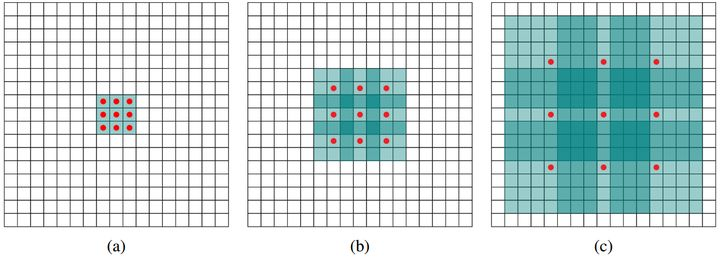
\includegraphics[width=.8\textwidth]{pics/dilation.jpg}
	\caption{Dilation Convolution}
	\label{fig:dilation}
\end{figure}

\subsection{1 $\times$ 1 Conv}
$1\times 1$卷积很显然,就是卷积核的长宽均为1,用$c_i$ 和$c_o$  分别表示输入和输出通道的数目,为了获得多个通道的输出,可以为每个输出通道创建一个形状为$c_i\times 1 \times 1$ 的卷积核张量,这样卷积核的形状是$c_o \times c_i \times 1 \times 1$。

由于$1\times 1$卷积的长宽为1,无法关注到周围像素的信息,只能关注到同一位置不同通道上的信息,其作用主要由以下几点:
\begin{itemize}
	\item 融合多个通道间的信息
	\item 在不改变feature map尺寸的情况下改变feature map的通道数,例如在图像分割中
	\item 降低参数量
	\item 在以每像素为基础应用时,$1\times 1$卷积相当于全连接层
\end{itemize}
更多解释可参考动手学深度学习:\href{https://zh-v2.d2l.ai/chapter_convolutional-neural-networks/channels.html#times-1}{$1\times 1$  卷积层}

\subsection{LSTM}

\subsection{GRU}